En este apéndice describiremos algunos pormenores de la construcción del conjunto de datos del Capítulo \ref{chap:05_dataset_creation}.


\section{Distribución de datos recolectados}
\label{app:distribucion_datos}
La Figura \ref{fig:fecha_articulos_por_medio_todas} muestra la distribución temporal de los artículos, sin aplicar ningún filtro por palabras, mientras que \ref{fig:fecha_articulos_por_medio_covid} muestra aquellas relacionadas al COVID-19 utilizando filtrando aquellos que mencionen alguna de las siguientes palabras: \emph{coronavirus, encierro, síntomas, covid, fase, fiebre, cuarentena, infectados, distanciamiento, normalidad,  Wuhan, aislamiento}. Podemos observar dos caídas. Hay un pequeño pozo en mayo 2020 que se debió a problemas técnicos de nuestros servidores de recolección. Por otro lado, observamos que algunos medios (particularmente La Nación) parecieran mencionar menos directamente al COVID (al menos con los términos referidos anteriormente) hasta un nuevo pico cerca de fin de año, coincidente con un nuevo rebrote del virus en este país. Sin embargo, estas mediciones pueden contener artefactos del método de filtrado: muchas notas contienen links a otras con sus títulos, pudiendo interferir en estas estimaciones.


\begin{figure}
    \centering
    \begin{subfigure}[t]{\textwidth}
        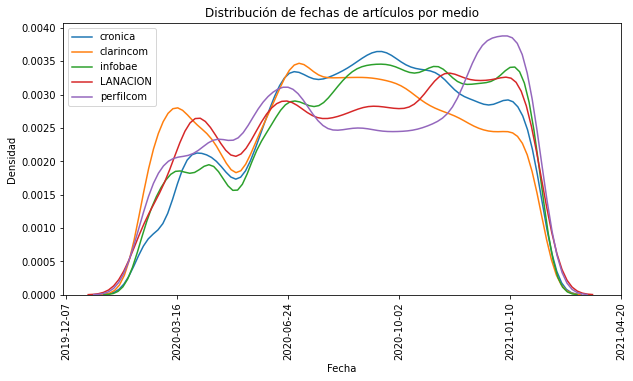
\includegraphics[width=\textwidth]{img/fechas_por_medios_todas.png}
        \caption{Distribución temporal de artículos recolectados, sin aplicar ningún filtro}
        \label{fig:fecha_articulos_por_medio_todas}
    \end{subfigure}

    \begin{subfigure}[t]{\textwidth}
        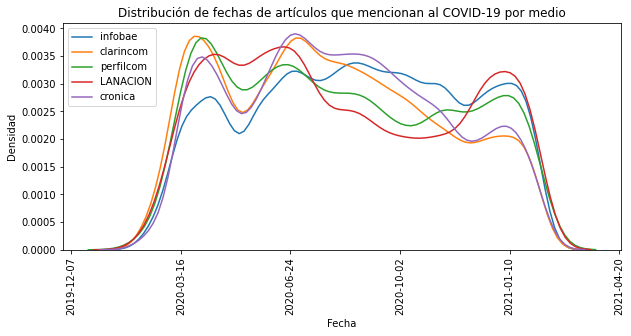
\includegraphics[width=\textwidth]{img/fechas_por_medios.png}
        \caption{Distribución temporal de artículos recolectados que mencionan COVID-19 o algún término relacionado}
        \label{fig:fecha_articulos_por_medio_covid}
    \end{subfigure}

    \caption{Gráficos de distribución de los datos recolectados.}
\end{figure}


\section{Recursos utilizados}

El etiquetado del conjunto de datos consumió alrededor de 450 horas de trabajo entre todos los anotadores. El gasto total de anotación fue de \num{125000} pesos argentinos, lo cual al tipo de cambio de ese entonces equivale a alrededor de \num{1400} dólares estadounidenses.

\section{Manual de criterios de anotación}
\label{app:manual_criterios_anotacion}
\chapter{Manual de criterios de anotación}
\label{app:manual_criterios_anotacion}
\section{Presencia de lenguaje discriminatorio}

Entendemos que hay discurso discriminatorio en el tweet si contiene declaraciones de carácter intenso y posiblemente irracional de rechazo, enemistad y aborrecimiento contra un individuo o contra un grupo, siendo estos objetivos de estas expresiones por poseer (o aparentar poseer) una característica protegida.

Este discurso puede manifestarse de manera explícita (insultos directos), celebraciones sobre asesinatos u otros crímenes, o bien otras expresiones más veladas. Lo que queremos captar es la intención del autor del tweet. El carácter discriminatorio de un mensaje está dado tanto por el contexto (en este caso, el tweet original del medio periodístico y posiblemente la nota) y el contenido del tweet en sí mismo. Por ejemplo, un comentario que diga “excelente” sin contexto es una cosa, y decir eso mismo en una nota que relata un femicidio, o un asesinato es otra muy distinta.

Las características protegidas que vamos a tener en cuenta son las siguientes:

\begin{enumerate}
\item Sexo (Mujeres, concretamente)
\item Género o identidad sexual (Colectivo LGBTI)
\item Ser inmigrantes, extranjeros, pueblos aborígenes u otras nacionalidades (Xenofobia, racismo)
\item Situación socioeconómica o por barrio de residencia
\item Poseer discapacidades, problemas salud mental o de adicción al alcohol u otros estupefacientes
\item Opinión o ideología política
\item Aspecto o edad (mayormente, gordofobia/gerontofobia)
\item Antecedentes penales o estar privado de la libertad

\end{enumerate}

Es decir, para considerar un mensaje como discriminatorio, debe cumplir que el discurso discriminatorio está orientado hacia un individuo o grupo de al menos una (aunque posiblemente más de una) característica protegida.


Consideramos que el mensaje del tweet (a la vez que el receptor del odio) es el que determina si puede o no ser considerado discriminatorio y hacia qué grupo está dirigido. Esto puede no necesariamente coincidir con el destinatario explícito del mensaje: por ejemplo, si alguien le dice a Susana Giménez “judía sionista hdp”, a pesar de no ser Susana Giménez judía, se puede considerar esto como discurso de odio contra las minorías religiosas y/o discurso xenófobo.


\section{Llamado a la acción}

Entendemos que un tweet (que contiene discurso discriminatorio) llama a la acción si contiene alguna incitación a tomar algún tipo de medida contra el sujeto o grupo ofendido. Esta medida puede ser de carácter violento (“hay que matarlos ya” “pongámosles una bomba”) o de carácter menos violento (“hay que dejar de comprarles a estos chinos ladrones”)

Estos tweets nos interesan particularmente porque son los más peligrosos y dañinos: los que llaman a tomar algún tipo de represalia contra la persona o el grupo en cuestión.

\section{Características protegidas}

Finalmente, para cada tweet deberemos marcar qué grupo o característica protegida es atacado. En este caso, necesariamente un grupo/característica debe ser seleccionado:

Usaremos una notación abreviada en la interfaz de etiquetado, en la que algunos de los grupos o características mencionadas fueron reagrupadas de la siguiente manera:

\begin{enumerate}
    \item MUJER: por su sexo
    \item LGBTI: por género o identidad sexual
    \item RACISMO: Por ser inmigrantes, extranjeros, pueblos aborígenes u otras nacionalidades (Xenofobia, racismo)
    \item POBREZA: Por situación socioeconómica o por barrio de residencia.
    \item DISCAPAC: Por tener discapacidades, problemas salud mental o de adicciones
    \item POLITICA: Por su opinión o ideología política
    \item ASPECTO: Por su aspecto o edad
    \item CRIMINAL: Por sus antecedentes o situación penal (presos)
\end{enumerate}

A su vez, agregamos la categoría “OTROS”. Esta categoría es excepcional, y debería utilizarse sólo si algún tipo de discriminación no está contemplado en estas categorías.

Respecto a la discriminación de carácter político tiene que ser algo más que una mera opinión  sino tener una componente irracional, de descalificación y de aborrecimiento considerable sobre un individuo o una facción política.

No se contempla dentro de las categorías protegidas a las profesiones. Es decir, no tenemos en cuenta el discurso contra científicos, médicos, o periodistas; de esto último hay bastante material agresivo en los comentarios.


\subsection{Lineamientos generales}

El discurso discriminatorio no es sólo discurso ofensivo contra una persona o grupo con alguna de las características protegidas. Tiene que apelar a su condición de mujer, inmigrante, LGBTI, etc. para que lo consideremos así.

Por ejemplo: si alguien agrede a una mujer, a un inmigrante, o a alguien de la comunidad LGBTI, no necesariamente está incurriendo en un discurso discriminatorio salvo que apele a algo que remita a su característica como tal.


Expresiones de aprobación ante noticias de crímenes o acciones contra persona o grupo de las características protegidas son consideradas discriminatorias.

\subsubsection{Ejemplos}

Violan a la reconocida actriz XXXX YYYY
Asesinan a un comerciante chino por creer que tenía Coronavirus
Motín y muerte en la prisión de Marcos Paz

Comentarios de contenido discriminatorio: (emoji de aplausos) - uno menos - bravo! -


Si no queda claro que haya un mensaje discriminatorio o parece de carácter difuso o demasiado tangencial, entonces etiquetar como no discriminatorio




\subsection{MUJER}

Insultar a una mujer sin hacer ninguna referencia particular a su condición de mujer no es suficiente para ser considerado discurso discriminatorio

Como regla: si el mismo insulto o agresión aplicase contra un hombre, entonces no debiéramos considerarlo como discriminación


Insultos contra las expresiones políticas del movimiento de las mujeres son consideradas en esta categoría: si se las insulta como feminazis, aborteras, pañuelito verde, etc



Apelaciones a su apariencia o aspecto propias de una mujer son consideradas en esta categoría. En este punto consideramos comentarios cosificadores


Insultar como “vieja” a una persona no califica como misoginia. Usar para ese caso la categoría ASPECTO que contempla la gerontofobia

EJEMPLOS:

Nati Jota furiosa por los comentarios que recibe en las redes.

Comentarios sexistas:

Pero si sos de plástico nena! (opina de manera denigratoria de su apariencia)
Flor de gato!
Miauuu!
A esta sólo se la conoce por su cuerpo y ahora se hace la santa. Andá a estudiar
Le damos hasta que San Lorenzo vuelva a Boedo
Y esta rubia tarada quién es?



Comentarios ofensivos pero no sexistas:
Callate forra (ofensivo pero no particularmente sexista)
Y esta quién es? A quién le importa?
Quién?
Nati cuánto?
Esta también recibe sobres?
Otra descerebrada más (súper agresivo, pero es un comentario que podría recibir un hombre, aunque en menor cantidad…)
Andá a cagar..boluda..conductora de 4ta..
HDP
Boba



\subsection{LGBTI}

Expresiones de disgusto o rechazo del estilo “qué asco” frente a integrantes de la colectividad deben ser marcados como discurso discriminatorio


Apelaciones a la anatomía o del estilo “biologicistas” deben ser marcados como discurso discriminatorio


Ejemplos:

Anibal Pachano sobre la cuarentena: “este virus nos está destruyendo a los actores”


Comentarios discriminatorios:

Qué asco este sujeto
Y a este trolo quién le pidió su opinión?
Me desagrada


Comentarios ofensivos pero no discriminatorios:

Ajá, y?
No me importa tu opinión, gracias
Se acuerdan cuando este atacaba a Cristina? Andá a llorarle al gato, Aníbal
Pelotudazo!


Famosa actriz trans dio una entrevista a La NACION: “Como mujer, estoy en la mejor etapa de mi vida”


Comentarios discriminatorios:

Muy lindo todo, pero sos hombre
“Mujer” dice jajajaj naciste y morirás macho
Qué asco este trolo
(emoji de asco)
Una mujer con sorpresa
Trava horrendo
Perdón pero qué nombre dice tu DNI?


Comentarios ofensivos pero no discriminatorios:

Quién?
Y a quién le interesa lo que diga esta mujer?
Que se vaya a cagar
Agradecele al gobierno de Néstor que tenés derechos





\subsection{RACISMO}

Asignar a todo un pueblo con una característica o actividad particular negativa entra en esta categoría
Cualquier llamada a expulsar, matar, tirar bombas, destruir, aniquilar, etc a un pueblo, inmigrantes o país entra en esta categoría. Más aún, deben ser marcadas como “llamadas a la acción”
Teorías conspirativas (hasta cierto punto) o acusaciones a un Gobierno/Estado no deberían entrar en esta categoría
¿Acusaciones respecto al virus?



Ejemplos:

Rescatan en China a cuarenta gatitos bebé que iban a ser utilizados en restaurantes


Comentarios discriminatorios:

Chinos asquerosos
Malparidos! Chinos de mierda
Sigan desparramando pestes hijos de puta!
Por qué no se comen entre ellos?
País horrible y enfermo
Estos chinos nos diseminan su peste por todo el mundo

Comentarios discriminatorios y que además llaman a la acción:

Son una plaga estos chinos, hay que matarlos a todos
Ojalá les caigan veinte bombas
Hay que barrer ese país de la faz de la tierra

Comentarios ofensivos pero no racistas:

Son comunistas, qué querés
Lo rescataron a Mauri?




Otros comentarios no racistas

El gobierno chino está intentando controlar todo, cuidado
Mienten con que controlaron el virus, cómo no van a mentir con esto también?
De terror!


Tomas de terrenos: se profundizan las tomas en todo Buenos Aires


Comentarios discriminatorios:

Rajen a todos los peruanos de las tomas! (llama a la acción, además)
Increíble, cualquier paraguayo o bolita de mierda te saca la casa

\subsection{POBREZA}

Expresiones denigrantes sobre la condición socioeconómica son consideradas discriminatorias: referirse a las personas sin empleo como “vagos”, a otros como “(chori)planeros”
Respecto a la gente que posee planes de asistencia social, si es una opinión general sin ser ofensiva no se considera discriminatoria (del estilo “hay que reducir el gasto social y los planes”, “perdieron la cultura del trabajo”)

Presupuesto: aumentó el gasto en planes asistenciales durante la pandemia

Ejemplos discriminatorios:

Basta de mantener vagos!
Cansada de los planeros
Che laburar estos atorrantes ni en pedo no?
PARASITOS

Ejemplos no discriminatorios

La gente que trabaja y aporta impuestos es cada vez menos. Estamos al horno



\subsection{POLITICA}

Apreciaciones derogatorias sobre la posición política son consideradas discriminatorias : zurdo/a, bolchevique, peroncho, gorila, kuka, etc
Acusaciones de corrupción o de “recibir sobres” no son consideradas discriminatorias
Tampoco aquellas expresiones que traten de inútiles a funcionarios
Tratar de viejo/a, gordo/a, u otras cuestiones físicas deben ser marcados en las categorías respectivas, no acá

Aumentó el gasto en planes asistenciales durante la pandemia

Ejemplos discriminatorios:

BASTA ZURDOS DE ROBARNOS
Bolcheviques de mierda

Ejemplos no discriminatorios

La gente que trabaja y aporta impuestos es cada vez menos. Estamos al horno
Qué gobierno de inútiles
Son unos delincuentes
Hijos de mil puta!
Siguen volando los sobres para el Congreso
Siga siga la impresión




\subsection{ASPECTO}

Apreciaciones denigrantes sobre la apariencia de una persona y/o su edad
Principalmente, tenemos en mente la gordofobia y gerontofobia, pero puede referir a otras características físicas (por ejemplo, la altura)
En casos en las cuales haya solapamiento con mujer, marcar ambas


Luis Brandoni: “No convoqué el banderazo”

Ejemplos discriminatorios:

Viejo de mierda!
Qué decrépito impresentable que es este señor
Estás gagá, pelotudo

Jorge Lanata vuelve a la televisión

Ejemplos discriminatorios:

Gordo chanta otra vez volvés a vender pescado podrido?
porque no te vas vos tambien con todos bola de sebo!!!1
Estás gagá, pelotudo









\subsection{CRIMINAL}

Cualquier comentario que celebre acciones contra criminales o personas privadas de su libertad (golpizas, asesinatos, muerte en motines, etc) entra en esta categoría
En este ítem muchas veces veremos que son llamados a la acción: el de “matarlos”, llamar a reducir sus derechos, etc
Muere un delincuente tras un enfrentamiento con la policía

Ejemplos discriminatorios:

Uno menos!
Excelente!
(emoji de aplausos)
Que pena, pobrecito

Ejemplos que además llaman a la acción

MUY BIEN! Felicitaciones al policía, hay que liquidarlos sin piedad


1...100 101..200 …. 501...600

Primera fase: Et 1 => 1..100, Et 2 => 101 .. 200 … Et 6 => 501..600
Segunda fase Et2 => 1..100 Et1 => 101..200…. Et 6 => 401..500 Et 5 => 501..600

Shufflear temporalmente

Ejemplos no discriminatorios


Cómo puede ser que nuestra Ministra no haga nada?
La policía actuó correctamente.

Motín por el Coronavirus en Olmos: 3 muertos

Ejemplos discriminatorios y que llaman a la acción

Hay que rociar con nafta todas las cárceles
Soltemos 3 o 4 infectados con COVID en cada cárcel y problema solucionado
Paredón y listo



\subsection{DISCAPACIDAD}

Referencias peyorativas de adicciones a drogas, alcohol u otros estupefacientes
También referencias peyorativas a la salud mental de la persona en cuestión
Decir “está loco” no entra acá :-)
Malena Pichot sale a cruzar a Baby Etchecopar
Ejemplos discriminatorios:

Callate faloperita!
Jorge Lanata vuelve a la televisión

Ejemplos discriminatorios:

Che no probaste dejar la merca gordo?

Noticia sobre Patricia Bullrich...

Ejemplos discriminatorios:

Largá la (emoji de botella) Pato
Borracha hdp



\subsection{OTROS}

Esta categoría está reservada para cualquier otro tipo de discriminación que no esté contemplada en las categorías mencionadas
Insultos a profesiones (científicos, periodistas, por ejemplo) no entran en este apartado
ESTA CATEGORIA ES SUMAMENTE EXCEPCIONAL. NO USAR INDISCRIMINADAMENTE
